% Frugal AI seminar, project 2: speech to a checked form (FrugalAI/code/voice-form). Procedure and theory, plus one
% frame of model-comparison results (script text only). CheatSheet-safe: no floats, the table is wrapped in adjustbox.

\section[Voice Form]{Project: Speak a Form}

%%%%%%%%%%%%%%%%%%%%%%%%%%%%%%%%%%%%%%%%%%%%%%%%%%%
\begin{frame}[fragile]\frametitle{}
\begin{center}
{\Large Project: Speak a Form}

\medskip
{\small (Marathi or Hindi speech in, a checked form out, on a laptop with no internet at run time)}
\end{center}
\end{frame}

%%%%%%%%%%%%%%%%%%%%%%%%%%%%%%%%%%%%%%%%%%%%%%%%%%%
\begin{frame}[fragile]\frametitle{Why Speak a Form?}
\begin{itemize}
\item Field workers fill long forms on a phone, often in a second language, often standing up.
\item Speaking is faster than typing in Devanagari (the script of Hindi and Marathi).
\item A form filled from speech is a structured record that any database can take.
\item Idea: use a small model only for the part that needs language, and plain code for everything that can be checked.
\end{itemize}
{\tiny (Ref: FrugalAI code/voice-form)}
\end{frame}

%%%%%%%%%%%%%%%%%%%%%%%%%%%%%%%%%%%%%%%%%%%%%%%%%%%
\begin{frame}[fragile]\frametitle{Procedure: Listen, Pick Fields, Check, Confirm}
\begin{center}
\adjustbox{max width=0.97\linewidth, max totalheight=0.26\textheight}{%
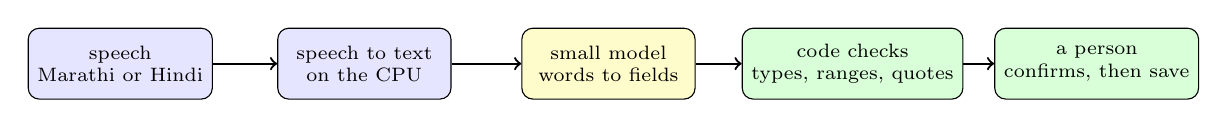
\begin{tikzpicture}
\tikzstyle{b}=[draw, rounded corners, align=center, minimum height=0.9cm, minimum width=2.2cm, font=\scriptsize]
\node[b, fill=blue!10] (s) at (0,0) {speech\\Marathi or Hindi};
\node[b, fill=blue!10] (t) at (3.1,0) {speech to text\\on the CPU};
\node[b, fill=yellow!20] (m) at (6.2,0) {small model\\words to fields};
\node[b, fill=green!15] (c) at (9.3,0) {code checks\\types, ranges, quotes};
\node[b, fill=green!15] (p) at (12.4,0) {a person\\confirms, then save};
\draw[->, thick] (s) -- (t);
\draw[->, thick] (t) -- (m);
\draw[->, thick] (m) -- (c);
\draw[->, thick] (c) -- (p);
\end{tikzpicture}}
\end{center}
\begin{itemize}
\item Speech to text: a speech model (IndicConformer from AI4Bharat, Whisper or Vosk) turns the audio into words.
\item The small model decides which words belong to which field, and must quote the words each value came from.
\item Plain code does the rest; the person has the last word.
\end{itemize}
{\tiny (Ref: FrugalAI code/voice-form)}
\end{frame}

%%%%%%%%%%%%%%%%%%%%%%%%%%%%%%%%%%%%%%%%%%%%%%%%%%%
\begin{frame}[fragile]\frametitle{Implementation: Who Does What}
\begin{center}
\scriptsize
\adjustbox{max width=\linewidth}{%
\begin{tabular}{p{0.46\linewidth}p{0.50\linewidth}}
\hline
Step & Done by \\
\hline
Speech to text & a speech model, swappable \\
Number words, dates, phone, blood pressure, options & plain code, tested \\
Which words are which field & the small model, quoting its evidence \\
Types, ranges, ``was this really said?'' & plain code \\
Follow-up questions for missing fields & plain code \\
Saving & plain code; refused until a person confirms \\
\hline
\end{tabular}}
\end{center}
\begin{itemize}
\item A form is one YAML file (a plain text settings file): fields, types, ranges, labels in English, Marathi and Hindi.
\item A new form needs no new code.
\end{itemize}
{\tiny (Ref: FrugalAI code/voice-form)}
\end{frame}

%%%%%%%%%%%%%%%%%%%%%%%%%%%%%%%%%%%%%%%%%%%%%%%%%%%
\begin{frame}[fragile]\frametitle{Which Small Model Reads the Words?}
\begin{center}
\scriptsize
\adjustbox{max width=\linewidth}{%
\begin{tabular}{p{0.30\linewidth}p{0.20\linewidth}p{0.18\linewidth}p{0.24\linewidth}}
\hline
Model & Marathi, fields right & Hindi, fields right & Seconds per line (about) \\
\hline
Qwen3 1.7B & 0.89 & 0.93 & 10 \\
Gemma 2 2B & 0.93 & 0.97 & 50 \\
Dhir 2B & 0.97 & 0.97 & 24 \\
\hline
\end{tabular}}
\end{center}
\begin{itemize}
\item 27 lines per language, one run each, on the text of the script (a perfect ear), not on real speech.
\item Dhir is the most accurate in Marathi and about 2.4 times slower than Qwen3; Gemma is the slowest but invents the fewest values (about 1 in 27 lines, against 5 to 7 for Dhir and Qwen3).
\item The engines differ (LM Studio, and llama-server for Dhir) and the PC was busy: compare the order, not the seconds.
\item Nothing is measured on real speech yet, and the line sets were drafted by Claude.
\end{itemize}
{\tiny (Ref: our runs, 26 October and 19 November 2026; FrugalAI code/voice-form README)}
\end{frame}

%%%%%%%%%%%%%%%%%%%%%%%%%%%%%%%%%%%%%%%%%%%%%%%%%%%
\begin{frame}[fragile]\frametitle{Design Rules and Safety}
\begin{itemize}
\item Offline at run time, after a one-time model download: any attempt by the app to reach another machine is blocked and counted.
\item Every value shows the words it came from, so a person can catch a misheard number.
\item Nothing is saved until a person confirms and every required field is valid.
\item Data entry only: no advice, no diagnosis, no dosing.
\item The forms are simplified demonstrations with made-up data, not official forms.
\end{itemize}
{\tiny (Ref: FrugalAI code/voice-form; docs/safety.md)}
\end{frame}
